\documentclass[12pt,a4paper]{exam}
\usepackage[utf8]{inputenc}
\usepackage[T1]{fontenc}
\usepackage{amsmath}
\usepackage{amsfonts}
%\usepackage{amssymb}
\usepackage{graphicx}
\usepackage{geometry}
\usepackage{enumitem}

\geometry{a4paper, margin=2cm}

\usepackage{cprotect}

\usepackage{xcolor}
\definecolor{maroon}{cmyk}{0, 0.87, 0.68, 0.32}
\definecolor{halfgray}{gray}{0.55}
\definecolor{ipython-frame}{RGB}{207, 207, 207}
\definecolor{ipython-bg}{RGB}{247, 247, 247}
\definecolor{ipython-red}{RGB}{186, 33, 33}
\definecolor{ipython-green}{RGB}{0, 128, 0}
\definecolor{ipython-cyan}{RGB}{64, 128, 128}
\definecolor{ipython-purple}{RGB}{170, 34, 255}
\usepackage{listings}
\lstdefinelanguage{iPython}{
	morekeywords={access,and,del,except,exec,in,is,lambda,not,or,raise},
	morekeywords=[2]{for,print,abs,all,any,basestring,bin,bool,bytearray,callable,chr,classmethod,cmp,compile,complex,delattr,dict,dir,divmod,enumerate,eval,execfile,file,filter,float,format,frozenset,getattr,globals,hasattr,hash,help,hex,id,input,int,isinstance,issubclass,iter,len,list,locals,long,map,max,memoryview,min,next,object,oct,open,ord,pow,property,range,reduce,reload,repr,reversed,round,set,setattr,slice,sorted,staticmethod,str,sum,super,tuple,type,unichr,unicode,vars,xrange,zip,apply,buffer,coerce,intern,elif,else,if,continue,break,while,class,def,return,try,except,import,finally,try,except,from,global,pass, True, False},
	sensitive=true,
	morecomment=[l]\#,%
	morestring=[b]',%
	morestring=[b]",%
	moredelim=**[is][\color{black}]{@@}{@@},
	identifierstyle=\color{black}\footnotesize\ttfamily,
	commentstyle=\color{ipython-cyan}\footnotesize\itshape\ttfamily,
	stringstyle=\color{ipython-red}\footnotesize\ttfamily,
	keepspaces=true,
	showspaces=false,
	showstringspaces=false,
	rulecolor=\color{ipython-frame},
	frame=single,
	frameround={t}{t}{t}{t},
	%framexleftmargin=6mm,
	%numbers=left,
	%numberstyle=\color{ipython-cyan},
	backgroundcolor=\color{ipython-bg},
	%   extendedchars=true,
	basicstyle=\footnotesize\ttfamily,
	keywordstyle=[2]\color{ipython-green}\bfseries\footnotesize\ttfamily, 
	keywordstyle=\color{ipython-purple}\bfseries\footnotesize\ttfamily
}

\lstdefinelanguage{iOutput} {
	sensitive=true,
	identifierstyle=\color{black}\small\ttfamily,
	stringstyle=\color{ipython-red}\small\ttfamily,
	keepspaces=true,
	showspaces=false,
	showstringspaces=false,
	rulecolor=\color{ipython-frame},
	basicstyle=\small\ttfamily,
}

\lstnewenvironment{ipython}[1][]{\lstset{language=iPython,mathescape=true,escapeinside={*@}{@*}}%
}{%
}

\lstnewenvironment{ioutput}[1][]{\lstset{language=iOutput,mathescape=true,escapeinside={*@}{@*}}%
}{%
}

\title{Financial Market Course 24/25\\ Exam}
\author{Prof. Simone Freschi, Prof. Matteo Sani}
\date{$16^{\mathrm{th}}$ July 2025}

\printanswers
%\noprintanswer
\begin{document}
\maketitle
%\addpoints{exam}
\begin{center}
\fbox{\fbox{\parbox{5.5in}{\centering
Answer the questions in the spaces provided. If you run out of room for an answer, continue on the page back.}}}
\end{center}

\begin{center}
\vspace{5mm}
\makebox[0.75\textwidth]{Student's name:\enspace\hrulefill}
\end{center}

\section*{Questions}
\vspace{.5cm}
\begin{questions}


\question 	Write the equation for the price in real terms and nominal terms of an Inflation Linked Bond.
\begin{enumerate}
\item In the chart \ref{prima} is described the dynamic of US nominal rates and Break-even between June 2023 and December 2023. Describe what could have happened and why to prices of 10y TIP (Treasury Inflation Protected Bonds).


\item In the chart \ref{seconda} is described the dynamic of US nominal rates and Break-even between March 2020 and December 2020. Describe what could have happened and why to prices of 10y TIP (Treasury Inflation Protected Bonds).

\end{enumerate}
\makeemptybox{5cm}

\newpage


% \begin{figure}[h]
%     \centering
%     \includegraphics[width=0.75\linewidth]{inflation2.png}
%     \caption{10y US nominal rate and 10y Break-even}
%     \label{seconda}
% \end{figure}

% \begin{figure}[h]
%     \centering
%     \includegraphics[width=0.75\linewidth]{inflation.png}
%     \caption{10y US nominal rate and 10y Break-even}
%     \label{prima}
% \end{figure}

\newpage



\question Describe what are the main characteristics of a Repo Contract. 
\begin{enumerate}
\item In the chart \ref{terza} is described the delivery Basket of the BTP Future March 2025 (IKH5) which is currently trading at 118.63. The bond BTPS 4.35 Nov33 is the cheapest to deliver with a price of 105.50 and a conversion factor of 0.8953. Describe if there is an arbitrage opportunity and what kind of strategy would you implement. (\textit{hint}: check the basis and use the cash and carry strategy) 

\begin{figure}[h]
    \centering
    \includegraphics[width=0.75\linewidth]{BondFuture.png}
    \caption{BTP March 2025 Futures}
    \label{terza}
\end{figure}

\end{enumerate}
\makeemptybox{5cm}



\question Describe the equation for the return attribution model by Brinson, Hood and Beebower (BHB). 
\begin{enumerate}[label=(\alph*),font=\itshape]
\item Explain the difference between Allocation Effect and Security Selection Effect 
\item Imagine that your portfolio is underweight Tech (10\% vs 20\% Benchmark) and the Tech sector is up 15\%. The Tech stocks in your portfolio are up only 25\%. Determine the allocation effect and the selection effect and the overall portfolio result wrt to sector.
\end{enumerate}
\makeemptybox{5cm}

\question
What should we put instead of the \texttt{?} to make the following boolean expression \texttt{True} ?
\begin{ipython}
True and False or ?
\end{ipython}
\makeemptybox{5cm}
\begin{solution}
You need \texttt{?=True} since the boolean operators have the same precedence so the expression is evaluated from left to right.
Hence
\begin{equation*}
  \begin{gathered}
    \underbrace{\texttt{True and False}}_{\texttt{False}}\texttt{ or ?} = \texttt{True} \\
    \texttt{False or ?} = \texttt{True} \implies \texttt{?} = \texttt{True} \\
    \end{gathered}
\end{equation*}
\end{solution}


%%%%%%%%%%%%%%%%%%%%%%%%%%%%%%%%%%%%%%%%%%%%%%%%%%%%%%%%%%
\question A portfolio has a daily return variation distribution as shown in the following figure. The picture also indicates the \textbf{5\% area} under the distribution. 
Based on the graph estimate the \textbf{2 days 95\%-VaR} and the \textbf{1 day 95\%-Expected Shortfall} values. 
Briefly justify the approximate numbers.
\begin{center}
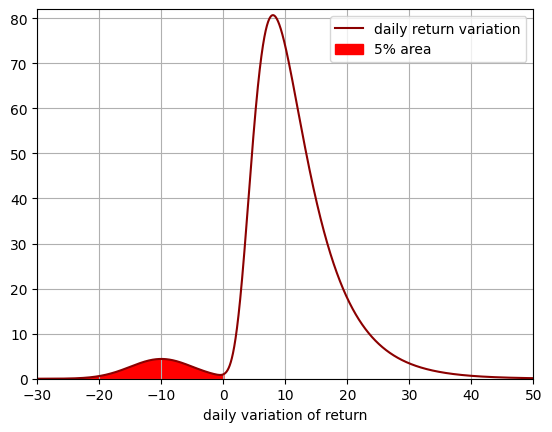
\includegraphics[width=0.8\textwidth]{var2}
\end{center}
\makeemptybox{3cm}

\begin{solution}
2 days 95\%-VaR $\approx 0 \cdot \sqrt{2}$, 1 day 95\%-ES $\approx 10$
\end{solution}

%%%%%%%%%%%%%%%%%%%%%%%%%%%%%%%%%%%%%%%%%%%%%%%%%%%%%%%%%%
\question
Company A finances itself by issuing a 5 year zero-coupon bond. Knowing that the bond is currently sold at \$ 83.75 and that similar riskless ZCB value is \$ 86.07, determine Company A default probability (assume the recovery rate to be 40\%).
\fillwithlines{3cm}
\begin{solution}
The bond price is related to the default probability $\delta$ through the following formula
\begin{equation*}
  P_{bond} = (1-\delta)P_{rf} + \delta P_{rf} R \implies \delta = \frac{P_{bond}-P_{rf}}{P_{rf}(R-1)}
\end{equation*}

Applying previous result to the problem gives a default probability of
\begin{equation*}
  \delta = \frac{83.75-86.07}{86.07\cdot(0.4-1)} \approx 4.49\% 
\end{equation*}
\end{solution}

%%%%%%%%%%%%%%%%%%%%%%%%%%%%%%%%%%%%%%%%%%%%%%%%%%%%%%%%%%
\question
Consider a portfolio whose efficient frontier is described by the following curve and assume that a risk-free investment yields $r_f = 10\%$.
\begin{center}
  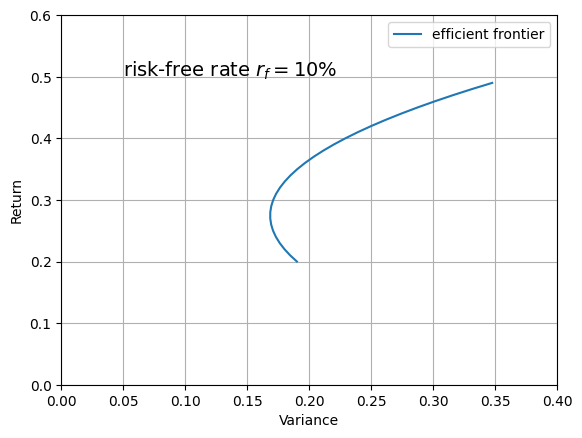
\includegraphics[width=0.7\linewidth]{efficient_frontier}
\end{center}
Using the plot determine the numerical value of the Sharpe ratio corresponding to the asset allocation of the portfolio maximizing it.
\fillwithlines{3cm}
\begin{solution}
In the Variance-Return plane the Sharpe portfolio can be identified by the tangent point between the efficient frontier and the CAL (the line passing through $(0.0, r_f)$. From the given plot this point lies approximately at $(0.2, 0.37)$ so
\begin{equation*}
  SR = \frac{r_P - r_f}{\sigma_P} = \frac{0.37-0.1}{0.4472} \approx 0.604
\end{equation*}
\end{solution}


\end{questions}
\end{document}

